\documentclass[11pt,a4paper]{article}

\usepackage[T1]{fontenc}
\usepackage[utf8]{inputenc}
\usepackage{lmodern}
\usepackage{amsmath,amssymb,amsfonts,amsthm}
\usepackage{geometry}
\usepackage{graphicx}
\usepackage{hyperref}
\usepackage{enumitem}


\geometry{margin=1in}
\setlist[itemize]{leftmargin=1.5em}

% --- Add these lines here ---
\theoremstyle{remark}
\newtheorem{remark}{Remark}
% ----------------------------


% --- Theorems and Propositions (Italicized text style) ---
\theoremstyle{plain}
\newtheorem{theorem}{Theorem}
\newtheorem{proposition}{Proposition}
\newtheorem{corollary}{Corollary}

\title{General Framework for Scalable Construction of Optimization Benchmark Functions}
\author{
	Khoirul Faiq Muzakka\(^{\ast\dagger}\),
	Others*, 
	Others*,
	Others*,
	Martin Finsterbusch\(^{\ast}\)\\
	\small \(^{\ast}\)Institute of Energy Materials and Devices (IMD-2)\\
	\small Forschungszentrum J\"ulich GmbH, Germany\\
	\small \(^{\dagger}\)Email: \href{mailto:k.muzakka@fz-juelich.de}{k.muzakka@fz-juelich.de}
}
\date{\today}

\begin{document}

\maketitle

\begin{abstract}
This paper proposes a general framework for constructing scalable families of
continuous optimization benchmark functions from known base functions. The
framework gives explicit construction prescriptions together with sufficient
conditions that preserve analytically known global optima. It is intended as a
programmable extension of existing benchmark suites, enabling many reproducible
problem instances with controlled landscape properties and known reference
optima. A C++ and Python implementation, \textsc{FuncCraft}, is provided to support
practical benchmark generation and future large-scale studies of algorithm
robustness.
\end{abstract}

\setcounter{tocdepth}{1}
\tableofcontents


\section{Introduction}
\label{sec:introduction}

Benchmark functions play a central role in the development and evaluation of
optimization algorithms. They provide controlled test problems for analyzing
convergence behavior, robustness, scalability, exploration--exploitation
trade-offs, and algorithmic performance under different landscape properties.
Consequently, benchmark suites such as the CEC competitions and the BBOB
testbed have become standard evaluation platforms for numerical optimization.

Despite their widespread use, existing benchmark suites share a common
limitation: they contain only a relatively small number of manually designed
benchmark functions. Typical benchmark collections consist of only a few dozen
problems with fixed landscape characteristics. While such benchmark suites are
indispensable for standardized comparison, they inevitably sample only a tiny
fraction of the enormous space of possible optimization landscapes. As a
result, an optimization algorithm may perform well on a particular benchmark
suite while exhibiting substantially different behavior on related, but
unrepresented, landscape structures.

This limitation becomes increasingly important as optimization algorithms become
more sophisticated. Modern optimization methods are often designed to be robust
across a wide variety of problem classes rather than being tailored to a small
collection of canonical functions. Consequently, robustness studies require
algorithms to be evaluated on hundreds or even thousands of diverse benchmark
instances, rather than on only a few dozen manually constructed problems.
Achieving such large-scale evaluation is difficult if every benchmark function
must be designed individually.

The primary objective of this work is therefore not to introduce another
benchmark suite, but to develop a general mathematical framework for benchmark
function construction. Instead of manually designing individual benchmark
functions, we seek a systematic methodology for generating large families of
optimization problems from a collection of known base functions while preserving
important analytical properties, most notably the location and value of the
global optimum.

More specifically, the proposed framework views benchmark construction as a
sequence of three independent design stages. First, coordinate transformations
modify the geometry of the search space through operations such as shifting,
rotation, scaling, conditioning, subspace selection, or nonlinear warping.
Second, value transformations reshape the objective values of individual
components, allowing the construction of plateaus, repeated minima,
oscillations, saturation, or additional local minima while preserving known
global optima whenever desired. Finally, a composition function combines the
transformed components into the final objective function, controlling the
interaction among component landscapes, spatial dominance, basin hierarchy,
deception, and multimodality.

This decomposition naturally separates benchmark design into three independent
questions:
\begin{enumerate}
	\item How should the search-space geometry be modified?
	\item How should the landscape of each component be reshaped?
	\item How should the transformed components interact?
\end{enumerate}
Rather than treating these operations independently for each benchmark
function, the proposed framework provides a unified mathematical formalism in
which each operation is represented explicitly and can be analyzed separately.

The proposed three-stage decomposition serves both as a constructive framework
for benchmark generation and as a natural taxonomy for benchmark
classification. On the constructive side, each stage can be extended
independently without modifying the overall framework: new coordinate
transformations, value transformations, or composition functions can be
incorporated simply by introducing new instances of the corresponding
construction ingredients. Consequently, the framework should be viewed as a design language
for optimization landscapes rather than as a fixed benchmark collection. At
the same time, the same decomposition provides a systematic classification of
generated benchmark functions. Instead of assigning an arbitrary name to each
generated instance, a benchmark can be characterized by its underlying base
functions together with its coordinate-transformation class,
value-transformation class, and composition-function class. This structural
representation separates the general construction recipe from its numerical
parameters and random seed, enabling large benchmark collections to be
organized into meaningful families, compared according to their dominant
landscape mechanisms, and reproduced exactly through associated metadata.


The framework also establishes sufficient conditions under which the generated
benchmark function retains a known global optimum. This provides theoretical
guarantees that are essential for optimization benchmarking, where objective
errors, success rates, and convergence behavior must be evaluated with respect
to a known optimum. Beyond preserving known optima, the framework also provides
systematic prescriptions for constructing benchmark functions with prescribed
landscape characteristics, including multimodality, deceptive basins,
nonseparability, ill-conditioning, variable interaction, repeated optima, and
hierarchical compositions.

To facilitate practical use of the proposed methodology, we provide both C++
and Python implementations in an open-source software package called
\textsc{FuncCraft}. Rather than supplying a fixed collection of benchmark
functions, \textsc{FuncCraft} enables users to generate arbitrarily many
benchmark instances by combining different coordinate transformations, value
transformations, and composition functions. This enables large-scale robustness
studies involving hundreds or thousands of benchmark functions generated from a
common mathematical framework.

The primary contribution of this paper is the development of the mathematical
and computational foundation underlying this framework. We establish general
minimum-preservation conditions, develop constructive prescriptions for
benchmark generation, analyze the roles of the individual construction
ingredients, and show how the same construction decomposition induces a natural
classification of generated functions. We further provide a structured labeling and metadata
scheme for organizing large benchmark collections and reproducing individual
instances exactly. Extensive benchmarking of optimization algorithms on large
collections of automatically generated functions is beyond the scope of the
present paper and will be reported in a separate companion study.


% --------------------------------------------------------------------------
\section{A General Composition Framework}
\label{sec:general-composition}
% --------------------------------------------------------------------------

The objective of this work is to construct new benchmark functions from a
given collection of known objective functions, referred to as
\emph{base functions}. The construction is required to satisfy two main
requirements. First, the global optimum of the generated function should remain
known analytically. Second, the construction should provide mechanisms for
controlling landscape properties such as multimodality, separability,
conditioning, variable interaction, basin geometry, and deceptiveness.

The starting point of benchmark construction is a set of base functions, such
as Rastrigin, Rosenbrock, and Ackley. Let \(D\) be the search dimension and let
\(\Omega\subseteq\mathbb{R}^D\) be the search domain. Suppose that there are
\(m\) base functions. A base function may act on all variables or only on a
lower-dimensional component space:
\[
\tilde g_i:\Omega_i\subseteq\mathbb{R}^{n_i}\to\mathbb{R},
\qquad i=1,\ldots,m,
\qquad n_i\le D.
\]
Each \(\tilde g_i\) has a known global minimizer and minimum value,
\[
x_i^\star\in\operatorname*{arg\,min}_{x\in\Omega_i}\tilde g_i(x),\qquad 
\tilde g_i^\star
=
\tilde g_i(x_i^\star).
\]
It is convenient to work with base functions whose minimum value is zero. We
therefore define
\[
g_i(y)
=
\tilde g_i(y)-\tilde g_i^\star.
\label{eq:bias-corrected-base}
\]
such that
\[
g_i(y)\ge g_i(x_i^\star) =0
\qquad\forall y\in\Omega_i,
\]
Thus each shifted function has known minimum value zero. From now on, unless
otherwise indicated, we call \(g_i\) the base function.

In constructing the benchmark function, we first specify a pointwise composition
function that maps the current point and the component values to the final
objective value:
\[
	\psi:\Omega\times\mathbb{R}^m\to\mathbb{R},
	\qquad
	(x,z)\mapsto \psi(x,z).
\]
Equivalently, for each \(x\in\Omega\), \(\psi_x(z)=\psi(x,z)\) is a
composition rule acting on the component-value vector. Once \(\psi\) is fixed,
it induces a function-level operator
\[
	\Psi_\psi:\mathcal{F}^m\to\mathcal{F},
	\qquad
	\mathcal{F}=\{h:\Omega\to\mathbb{R}\},
\]
by
\[
	\Psi_\psi(z_1,\ldots,z_m)(x)=\psi(x,z_1(x),\ldots,z_m(x)).
\]
Specifically, we consider generated functions of the form
\begin{equation}
\boxed{
	f(x)
	=
	\psi
	\left(
	x,
	\phi_1\!\left(g_1(T_1(x))\right),
	\ldots,
	\phi_m\!\left(g_m(T_m(x))\right)
	\right),
}
\label{eq:general-composition}
\end{equation}
where
\[
T_i:\Omega\to\Omega_i, \qquad
\phi_i:\mathbb{R}_{\ge0}\to\mathbb{R}, \qquad
\psi:\Omega\times\mathbb{R}^m\to\mathbb{R}
\]
are a coordinate transformation, a value transformation applied to the \(i\)-th
base function, and a composition function that combines the current point with
the transformed component values, respectively.

The three levels in \eqref{eq:general-composition} play distinct roles. The
coordinate transformation $T_i$ modifies the input geometry of the $i$-th
component. It may introduce shifting, rotation, scaling, subspace selection,
or nonlinear warping. The value transformation $\phi_i$ modifies the output
scale and shape of the $i$-th component. It may change curvature, growth rate,
flatness, or saturation. The composition function $\psi$ acts on the current
point and the component-value vector. It therefore determines how the component
landscapes interact and, when it depends explicitly on \(x\), how this
interaction changes across the search domain.

The main question is to identify conditions on $T_i$, $\phi_i$, and $\psi$
under which the generated function still has a known global minimizer.




\begin{proposition}[Nonnegative-function minimizer]
	\label{f_helper}
	Let \(h:\Omega\to\mathbb{R}\). Suppose there exists a known point
	\(x^\star\in\Omega\) such that
	\[
	h(x^\star)=0, \qquad
	h(x)\ge0
	\qquad
	\forall x\in\Omega.
	\]
	Then
	\[
	x^\star\in\operatorname*{arg\,min}_{x\in\Omega} h(x)
	\]
	and the global minimum value is \(0\).
\end{proposition}

\begin{proof}
	Since \(h(x)\ge0=h(x^\star)\) for all \(x\in\Omega\), the claim follows.
\end{proof}

This elementary observation is the backbone of the construction. The rest of
this section shows how to choose the three ingredients in
\eqref{eq:general-composition} so that the generated function satisfies the two
conditions in Proposition~\ref{f_helper}: zero value at a prescribed point and
nonnegativity everywhere.

\begin{proposition}[\(\psi\)-condition for minimum preservation]
	\label{thm:general-minimum-preservation}
	Let
	\[
	z_i(x)
	=
	\phi_i(g_i(T_i(x))),
	\qquad i=1,\ldots,m,
	\]
	and let \(\bar x\in\Omega\) be a candidate prescribed minimizer. Choose a
	composition function \(\psi:\Omega\times\mathbb{R}^m\to\mathbb{R}\) so that
	\[
	\psi(\bar x,z_1(\bar x),\ldots,z_m(\bar x))=0,
	\]
	and
	\[
	\psi(x,z_1(x),\ldots,z_m(x))\ge0
	\qquad
	\forall x\in\Omega.
	\]
	Then the generated function \(f(x)=\psi(x,z_1(x),\ldots,z_m(x))\) satisfies
	\[
	\bar x\in\operatorname*{arg\,min}_{x\in\Omega} f(x),
	\]
	and the global minimum value is \(0\).
\end{proposition}

\begin{proof}
	This follows immediately from Proposition~\ref{f_helper}, applied to
	\(h=f\). 
\end{proof}

\begin{remark}
	The conditions in Proposition~\ref{thm:general-minimum-preservation} are
	sufficient, but not necessary. The proposition gives a condition on
	\(\psi\) on the reachable pairs \((x,z(x))\): the candidate point must be
	mapped to zero, and every reachable pair must be mapped to a nonnegative
	value. Thus, Proposition~\ref{thm:general-minimum-preservation} should be interpreted as
	a practical sufficient condition for constructing benchmark functions with a
	known optimum, not as a complete characterization of all possible
	minimum-preserving compositions.
\end{remark}


Proposition~\ref{thm:general-minimum-preservation} places the final
responsibility on the composition function \(\psi\). To make that condition
easy to verify, we next impose a simple requirement on each value
transformation. This ensures that every transformed component remains a
nonnegative function with a known zero at the base-function minimizer.

\begin{proposition}[\(\phi_i\)-condition for preserving component minima]
	\label{prop:minimum-preserving-value-transformations}
	Let \(g_i:\Omega_i\to\mathbb{R}\) be a base function with known minimizer
	\(x_i^\star\) and minimum value \(0\), as defined above:
	\[
	g_i(x_i^\star)=0,
	\qquad
	g_i(y)\ge0
	\qquad
	\forall y\in\Omega_i.
	\]
	If the value transformation \(\phi_i:\mathbb{R}_{\ge0}\to\mathbb{R}\)
	satisfies
	\[
	\phi_i(0)=0,
	\qquad
	\phi_i(u)\ge0
	\qquad
	\forall u\ge0,
	\]
	then \(x_i^\star\) is a global minimizer of the transformed component
	\[
	z_i(y)=\phi_i(g_i(y)),
	\]
	with minimum value \(0\). That is,
	\[
	z_i(x_i^\star)=0,
	\qquad
	z_i(y)\ge0
	\qquad
	\forall y\in\Omega_i.
	\]
\end{proposition}

\begin{proof}
	At the known minimizer,
	\[
	z_i(x_i^\star)
	=
	\phi_i(g_i(x_i^\star))
	=
	\phi_i(0)
	=
	0.
	\]
	For any \(y\in\Omega_i\), the base function satisfies
	\(g_i(y)\ge0\). Since \(\phi_i(u)\ge0\) for all \(u\ge0\),
	\[
	z_i(y)
	=
	\phi_i(g_i(y))
	\ge0.
	\]
	Proposition~\ref{f_helper}, applied on \(\Omega_i\) with \(h=z_i\), then
	implies that \(x_i^\star\) is a global minimizer of \(z_i\).
\end{proof}

\begin{proposition}[Minimum preservation under coordinate pullback]
	\label{prop:coordinate-pullback-minimum}
	Let \(g:\Omega_g\to\mathbb{R}\), let \(T:\Omega\to\Omega_g\), and define
	\[
	h(x)=g(T(x)).
	\]
	If \(y^\star\) is a global minimizer of \(g\) on \(\Omega_g\), and if
	\(x^\star\in\Omega\) satisfies
	\[
	T(x^\star)=y^\star,
	\]
	then \(x^\star\) is a global minimizer of \(h\) on \(\Omega\).
	
	If \(y^\star\) is a local minimizer of \(g\) on \(\Omega_g\), \(T\) is
	continuous at \(x^\star\), and \(T(x^\star)=y^\star\), then \(x^\star\) is a
	local minimizer of \(h\) on \(\Omega\).
\end{proposition}

\begin{proof}
	For the global statement, \(g(y)\ge g(y^\star)\) for all \(y\in\Omega_g\).
	Since \(T(x)\in\Omega_g\) for all \(x\in\Omega\),
	\[
	h(x)=g(T(x))\ge g(y^\star)=g(T(x^\star))=h(x^\star),
	\]
	so \(x^\star\) is a global minimizer of \(h\).
	
	For the local statement, let \(V\subseteq\Omega_g\) be a neighborhood of
	\(y^\star\) on which
	\[
	g(y)\ge g(y^\star)
	\qquad
	\forall y\in V.
	\]
	By continuity of \(T\) at \(x^\star\), there exists a neighborhood
	\(U\subseteq\Omega\) of \(x^\star\) such that \(T(x)\in V\) for all
	\(x\in U\). Hence, for all \(x\in U\),
	\[
	h(x)=g(T(x))\ge g(y^\star)=h(x^\star),
	\]
	and \(x^\star\) is a local minimizer of \(h\).
\end{proof}

\begin{remark}
	The global statement assumes that \(y^\star\) is a minimizer of \(g\) on the
	whole target domain sampled by \(T\). This distinction matters on bounded
	domains. The transformed function does not sample \(g\) on an abstract
	reference region, but on the image set \(T(\Omega)\):
	\[
	\min_{x\in\Omega} g(T(x))
	=
	\min_{y\in T(\Omega)} g(y).
	\]
	If \(g\) is only known or intended to be minimized on a smaller reference
	region, then changing \(T\) may move points in \(\Omega\) into parts of the
	base landscape that were previously outside that region. In that case, a
	coordinate transformation can bring a deeper basin into the feasible search
	domain and change the effective global minimum. Benchmark constructions
	therefore need either a global minimum known on the full sampled target
	domain, or an explicit restriction on \(T(\Omega)\).
\end{remark}

With the component value transformations and coordinate pullbacks fixed, the
remaining design question is how to combine the prescribed component values.
The next proposition is the general prescribed-point construction: components
may be assigned to one or more prescribed points, and the resulting
component-value vectors are then passed to \(\psi\). This separates the
geometric placement of component minima from the final decision, made by
\(\psi\), about which prescribed points become global or local minima.

\begin{proposition}[Construction from prescribed points]
	\label{thm:prescribed-point-construction}
	Let
	\[
	z_i(x)=\phi_i(g_i(T_i(x))),
	\qquad
	z(x)=(z_1(x),\ldots,z_m(x)),
	\]
	where the value transformations satisfy
	Proposition~\ref{prop:minimum-preserving-value-transformations}. Let
	\(\tilde x_1,\ldots,\tilde x_r\in\Omega\) be prescribed points, and assign
	each component to one prescribed point by a map
	\[
	\sigma:\{1,\ldots,m\}\to\{1,\ldots,r\}.
	\]
	Assume that
	\[
	T_i(\tilde x_{\sigma(i)})=x_i^\star,
	\qquad i=1,\ldots,m.
	\label{eq:prescribed-point-assignment}
	\]
	For each \(k=1,\ldots,r\), set
	\[
	v^{(k)}=z(\tilde x_k).
	\label{eq:prescribed-component-vector}
	\]
	Choose \(\psi\) such that
	\[
	\psi(x,z(x))\ge0
	\qquad
	\forall x\in\Omega.
	\]
	Then the following statements hold for each prescribed point \(\tilde x_k\).
	
	\begin{enumerate}
		\item If \(\psi(\tilde x_k,v^{(k)})=0\), then \(\tilde x_k\) is a global
		minimizer of \(f\).
		
		\item If there exists a neighborhood \(U_k\subseteq\Omega\) of
		\(\tilde x_k\) such that
		\[
		\psi(\tilde x_k,v^{(k)})
		\le
		\psi(x,z(x))
		\qquad
		\forall x\in U_k,
		\label{eq:prescribed-point-local-condition}
		\]
		then \(\tilde x_k\) is a local minimizer of \(f\). If
		\(\psi(\tilde x_k,v^{(k)})>0\), it is a suboptimal local minimizer.
	\end{enumerate}
\end{proposition}

\begin{proof}
	First consider the components assigned to \(\tilde x_k\). If
	\(\sigma(i)=k\), then
	\[
	T_i(\tilde x_k)=x_i^\star.
	\]
	By Proposition~\ref{prop:minimum-preserving-value-transformations},
	\(x_i^\star\) is a global minimizer with value \(0\) of
	\(\phi_i\circ g_i\). Proposition~\ref{prop:coordinate-pullback-minimum}
	then implies that \(\tilde x_k\) is a global minimizer with value \(0\) of
	the pulled-back component \(z_i(x)=\phi_i(g_i(T_i(x)))\). In particular,
	\(z_i(\tilde x_k)=0\).
	Thus the assignment condition determines which entries of
	\(v^{(k)}=z(\tilde x_k)\) vanish.
	
	By definition of \(f\) and \(v^{(k)}\),
	\[
	f(\tilde x_k)=\psi(\tilde x_k,v^{(k)}).
	\]
	If this value is zero, then
	Proposition~\ref{thm:general-minimum-preservation}, applied with
	\(\bar x=\tilde x_k\), implies that \(\tilde x_k\) is a global minimizer.
	
	Finally, condition
	\eqref{eq:prescribed-point-local-condition} is exactly
	\[
	f(\tilde x_k)\le f(x)
	\qquad
	\forall x\in U_k.
	\]
	Hence \(\tilde x_k\) is a local minimizer. If its value is positive, it lies
	above the global minimum value zero and is therefore suboptimal.
\end{proof}

Finally, the same logic can be applied recursively. Once a generated function
has known minimum value zero and a known minimizer, it can itself be treated as
a base function in a higher-level composition.

\begin{proposition}[Nested construction]
	\label{prop:nested-construction}
	Let
	\[
	F_j:\Omega\to\mathbb{R},
	\qquad j=1,\ldots,r,
	\]
	be functions generated by the framework, each with known minimizer
	\(\xi_j^\star\) and minimum value \(0\):
	\[
	F_j(\xi_j^\star)=0,
	\qquad
	F_j(\xi)\ge0
	\qquad
	\forall \xi\in\Omega.
	\]
	Then the functions \(F_j\) may be used as base functions in a further
	composition layer. In particular, define
	\[
	H(x)
	=
	\psi_{\mathrm{out}}
	\left(
	x,
	\Phi_1(F_1(S_1(x))),
	\ldots,
	\Phi_r(F_r(S_r(x)))
	\right),
	\]
	where
	\[
	S_j:\Omega\to\Omega,
	\qquad
	\Phi_j:\mathbb{R}_{\ge0}\to\mathbb{R},
	\qquad
	\psi_{\mathrm{out}}:\Omega\times\mathbb{R}^r\to\mathbb{R}.
	\]
	If these maps satisfy the corresponding minimum-preservation conditions
	above, then the nested function \(H\) again has a known global minimum value
	\(0\).
\end{proposition}

\begin{proof}
	Each \(F_j\) has the same properties required of a base function in the
	preceding propositions: it is nonnegative and has known minimum value \(0\).
	Thus \(F_j\) can replace \(g_i\) in the construction. Applying
	Proposition~\ref{prop:minimum-preserving-value-transformations} to
	\(\Phi_j\circ F_j\), and then applying
	Proposition~\ref{thm:general-minimum-preservation} to the outer composition
	function \(\psi_{\mathrm{out}}\), gives the claim.
\end{proof}


Together, the propositions give a construction pipeline. First, the base
functions are shifted to have minimum value zero. Second, the value
transformations preserve this zero and nonnegativity. Third, the coordinate
transformations place component minima at prescribed points. Finally, the
composition function \(\psi\) assigns the final objective values and determines
which prescribed points are global minimizers, local minimizers, or neither.



\section{Analysis of Benchmark Construction Ingredients}

The previous section established the mathematical infrastructure needed to
construct functions with known global optima. This section turns to the design
question: once the optimum is protected, how do the choices of \(T_i\),
\(\phi_i\), and \(\psi\) shape the rest of the landscape? The discussion is
organized around two recurring issues: whether existing local minima are
preserved and how their shape changes, and whether the construction can generate
new local minima. As a first orientation, Table~\ref{tab:property-control}
summarizes which part of the construction is usually responsible for each
landscape property.

\begin{table}[t]
	\centering
	\caption{Typical landscape properties and the construction ingredient that
	primarily controls them.}
	\label{tab:property-control}
	\begin{tabular}{ll}
		\hline
		Property & Controlled by \\
		\hline
		Shift & \(T_i\) \\
		Rotation & \(T_i\) \\
		Conditioning & \(T_i\) \\
		Separability & \(T_i\) \\
		Multimodality & \(\phi_i,\psi\) \\
		Deceptive basins & \(\psi\) \\
		Repeated optima & \(\phi_i,\psi\) \\
		Funnels & \(\psi\) \\
		Hierarchy & \(\psi\) \\
		Plateaus & \(\phi_i\) \\
		Oscillations & \(\phi_i\) \\
		Dimensional embedding & \(T_i\) \\
		Recursive compositions & nested construction \\
		\hline
	\end{tabular}
\end{table}

The assignments in the table should be read as primary influences rather than
exclusive ones. These mechanisms can interact: \(T_i\) may change separability
before \(\psi\) couples the transformed components, and a nonmonotone
\(\phi_i\) may introduce local structure that is then amplified or suppressed
by \(\psi\). The subsections below therefore analyze the three choices
separately, starting from derivative and Hessian relations and then discussing
their consequences for preservation, shape change, and generation of new local
minima.

\subsection{Coordinate transformations $T_i$}
\label{subsec:coordinate-transformations}


The coordinate transformation \(T_i:\Omega\to\Omega_i\) determines where and how
the \(i\)-th base function is embedded in the full search space.
Proposition~\ref{prop:coordinate-pullback-minimum} gives the basic preservation
principle: if \(T_i\) maps a prescribed point to a component minimizer, then
the corresponding pulled-back component has a minimizer at the prescribed
point, provided the minimum is valid on the part of the base landscape sampled
by \(T_i(\Omega)\). This subsection looks beyond that minimum-preservation
statement and analyzes how \(T_i\) changes local shape, changes the sampled
region, or generates additional local minima.
Consider a single transformed component
\[
h(x)=g(T(x)).
\]
Assume first that \(g\) and \(T\) are differentiable. The first derivative is
\begin{equation}
	\nabla h(x)=J_T(x)^T\nabla g(T(x)).
	\label{eq:gradient-coordinate-transform}
\end{equation}
If \(g\) and \(T\) are twice differentiable, then
\begin{equation}
	\nabla^2 h(x)
	=
	J_T(x)^T\nabla^2 g(T(x))J_T(x)
	+
	\sum_{\ell}
	\frac{\partial g}{\partial y_\ell}(T(x))\nabla^2 T_\ell(x).
	\label{eq:hessian-nonlinear-transform}
\end{equation}

These two formulas describe the unconstrained local behavior, so the usual
stationary-point interpretation requires an interior basin. Suppose
\(x^\star\) is an interior point of the feasible domain, \(y^\star=T(x^\star)\)
is an interior local minimizer of \(g\), and \(g\) is differentiable at
\(y^\star\). Then
\[
	\nabla g(y^\star)=0,
\]
and \eqref{eq:gradient-coordinate-transform} gives
\[
	\nabla h(x^\star)
	=
	J_T(x^\star)^T\nabla g(y^\star)
	=
	0.
\]
Thus the preservation of the local minimum is consistent with the first
derivative analysis. The same conclusion also follows directly from values: if
\(T\) is continuous, then for all \(x\) sufficiently close to \(x^\star\),
\[
g(T(x))\ge g(T(x^\star)).
\]
Hence \(x^\star\) is a local minimizer of \(h=g\circ T\). If the minimum of
\(g\) is strict, the pulled-back minimum is strict only when the preimage of
\(y^\star\) is locally isolated; otherwise the transformation may produce a
flat set of minimizers. If \(x^\star\) or \(y^\star\) lies on a boundary, the
value argument still gives the correct feasible local-minimum statement, but
the unconstrained condition \(\nabla h(x^\star)=0\) need not hold.

The Hessian formula describes the change of shape in the same interior-basin
setting. Since \(\nabla g(y^\star)=0\), the second term in
\eqref{eq:hessian-nonlinear-transform} vanishes at \(x^\star\), so the
curvature becomes
\[
J_T(x^\star)^T\nabla^2 g(y^\star)J_T(x^\star).
\]
When \(J_T(x^\star)\) has full column rank, positive curvature of \(g\) is
preserved in the transformed variables, with changed orientation, scaling, and
conditioning. When \(J_T(x^\star)\) is rank deficient, some curvature directions
are lost, and an isolated minimum may become non-isolated or flat.

The same formulas also show how new stationary points can be generated. A point
\(x_0\) is stationary for \(h\) whenever
\[
J_T(x_0)^T\nabla g(T(x_0))=0.
\]
This may hold even if \(\nabla g(T(x_0))\ne0\), provided that the Jacobian of
\(T\) annihilates the descent direction of \(g\).
The second-order test is then applied to
\eqref{eq:hessian-nonlinear-transform}. In particular, positive definiteness of
\(\nabla^2h(x_0)\) on the relevant directions gives a strict local minimum.
This is the mechanism by which singular or nonlinear coordinate transformations
can create local minima that are not local minima of the original base function.
As an explicit example, consider a two-dimensional Sphere
\[
	g(y)=y_1^2+y_2^2,
\]
with unique minimizer \(y^\star=(0,0)\). Choose the nonlinear transformation
\[
	T(x_1,x_2)
	=
	\left(
	\frac{x_1^2-a^2}{s_1},
	\frac{x_2}{s_2}
	\right),
	\qquad
	a>0,
	\quad s_1,s_2>0.
\]
Then
\[
	h(x)=g(T(x))
	=
	\left(\frac{x_1^2-a^2}{s_1}\right)^2
	+
	\left(\frac{x_2}{s_2}\right)^2.
\]
The transformed function has two global minimizers,
\[
	(-a,0)
	\qquad\text{and}\qquad
	(a,0),
\]
because both points are mapped to \(y^\star\). Thus a non-injective
coordinate transformation can duplicate the optimum of a unimodal base
function and produce multiple basins even before any value transformation or
composition function is applied.
This is useful when repeated optima or deliberately duplicated basins are part
of the benchmark design. If the goal is a unique prescribed global minimizer,
however, such non-injective maps must be avoided or restricted so that the
preimage of the base optimum is unique in \(\Omega\).

A special case of coordinate transformation \(T_i\) which is of particular
interest is the affine map
\begin{equation}
	T_i(x)=A_i(x-\bar{x})+x_i^\star,
	\label{eq:affine-T}
\end{equation}
which places the component optimum \(x_i^\star\) at the prescribed point
\(\bar{x}\), since \(T_i(\bar{x})=x_i^\star\). Therefore, it satisfies the
condition in Proposition~\ref{prop:coordinate-pullback-minimum}: the component
minimum is pulled back to \(\bar{x}\). For
\[
h(x)=g(A(x-\bar{x})+x_g^\star),
\]
the derivative formulas reduce to
\begin{equation}
	\nabla h(x)=A^T\nabla g(T(x)),
	\qquad
	\nabla^2 h(x)=A^T\nabla^2 g(T(x))A.
	\label{eq:hessian-affine-transform}
\end{equation}
If \(A\) is nonsingular, local minima are preserved exactly: \(x_0\) is a local
minimum of \(h\) if and only if \(T(x_0)\) is a local minimum of \(g\). The
transformation changes the shape through the congruence
\(A^T\nabla^2 g(T(x))A\), so it can rotate, scale, and condition the local
landscape, but it does not create new local minima.

If \(A\) is singular or rank-deficient, then \(h\) only sees the restriction of
\(g\) to the affine image of \(T\). A point can therefore be a local minimum of
the restricted function even if it is not a local minimum of \(g\) in the full
component space. Such transformations can generate flat directions,
non-isolated minimizers, stationary manifolds, or additional local minima caused
by the removal of descent directions.

Figure~\ref{fig:coordinate-transform-sphere-3d} compares these cases on the
same Sphere base function. The affine transformation produces a single shifted,
rotated, and conditioned basin. The nonlinear folded transformation maps two
different points in the search space to the same base optimum, producing two
global basins from the same unimodal component.

\begin{figure}[t]
	\centering
	\includegraphics[width=\textwidth]{figures/coordinate_transform_sphere_3d.pdf}
	\caption{Coordinate transformations applied to the two-dimensional Sphere
	base function on \([-100,100]^2\). The affine transformation changes the
	location, orientation, and conditioning while preserving a single minimizer.
	The nonlinear folded transformation
	\(T(x_1,x_2)=((x_1^2-a^2)/s_1,x_2/s_2)\) duplicates the base optimum and
	creates two global minimizers.}
	\label{fig:coordinate-transform-sphere-3d}
\end{figure}

\subsection{Value transformations $\phi_i$}
\label{subsec:value-transformations}

The value transformation \(\phi_i\) acts after the coordinate-transformed base
value has been computed. Since the base functions are nonnegative and have
known minimum value zero, it is enough to study a single component of the form
\[
	h(x)=\phi(g(x)),
	\qquad
	g(x)\ge0,
	\qquad
	g(x^\star)=0.
\]
The basic preservation condition is
\[
	\phi(0)=0,
	\qquad
	\phi(u)\ge0
	\quad\text{for all }u\ge0.
\]
Under this condition, the known global minimizer of \(g\) remains a global
minimizer of \(\phi\circ g\). The remaining questions are how the local shape is
changed and whether additional local minima are introduced.

Assume first that \(g\) and \(\phi\) are differentiable. Then
\begin{equation}
	\nabla h(x)
	=
	\phi'(g(x))\nabla g(x).
	\label{eq:value-transform-gradient}
\end{equation}
If both are twice differentiable, then
\begin{equation}
	\nabla^2 h(x)
	=
	\phi''(g(x))\nabla g(x)\nabla g(x)^T
	+
	\phi'(g(x))\nabla^2 g(x).
	\label{eq:value-transform-hessian}
\end{equation}


Now suppose that the preserved point \(x^\star\) is an unconstrained interior
local minimizer of \(g\), that is, \(x^\star\) lies at the bottom of a smooth
local basin rather than only on the boundary of the feasible domain. Then
\(\nabla g(x^\star)=0\). Since \(g(x^\star)=0\), the first derivative becomes
\[
	\nabla h(x^\star)
	=
	\phi'(0)\nabla g(x^\star)
	=
	0.
\]
Thus the preserved minimizer is also a stationary point of the unconstrained
transformed function. The Hessian formula reduces to
\begin{equation}
	\nabla^2 h(x^\star)
	=
	\phi'(0)\nabla^2 g(x^\star).
	\label{eq:value-transform-hessian-minimizer}
\end{equation}
Because \(\phi(0)=0\) and \(\phi(u)\ge0\) for \(u\ge0\), differentiability at
the origin gives \(\phi'(0)\ge0\). Hence \(\phi'(0)\) acts as a curvature
weight at the preserved optimum. If \(\phi'(0)>0\) and
\(\nabla^2 g(x^\star)\) is positive semidefinite, then
\(\nabla^2 h(x^\star)\) is also positive semidefinite. If the scaled Hessian is
positive definite, the Hessian analysis confirms that \(x^\star\) remains at
the bottom of a local basin. If \(\phi'(0)=0\), the basin is flattened to
second order. If \(\phi'(0)\) is large or singular, the basin becomes sharper
or possibly nonsmooth.


The Hessian analysis describes the local structure at the preserved global
minimum. For other local minimizers, the situation is different. At a local
minimizer \(x_0\ne x^\star\), the value \(g(x_0)\) is generally positive, so
the local curvature of \(h\) depends on both \(\phi'(g(x_0))\) and
\(\phi''(g(x_0))\) through \eqref{eq:value-transform-hessian}. A local basin of
\(g\) can therefore be weakened, flattened, turned into a local maximum, or
reshaped into a different stationary structure unless \(\phi\) satisfies
additional monotonicity and curvature conditions near the value \(g(x_0)\).

There is, however, an important class of transformations that preserves local
minima. When \(\phi\) is strictly increasing on \(\mathbb{R}_{\ge0}\), it preserves the
ordering of values:
\[
	g(x_1)<g(x_2)
	\quad\Longrightarrow\quad
	\phi(g(x_1))<\phi(g(x_2)).
\]
Consequently, local minima are preserved exactly: a point is a local minimizer
of \(g\) if and only if it is a local minimizer of \(\phi\circ g\). Such
transformations change scale, curvature, and growth rate, but they do not create
new local minima by themselves. Typical examples are
\[
	\phi(u)=\alpha u,
	\qquad
	\phi(u)=\alpha u^p,
	\qquad
	\phi(u)=\log(1+\alpha u),
\]
with parameters chosen so that \(\phi(0)=0\), \(\phi(u)\ge0\), and \(\phi\) is
increasing on the relevant range. Linear scaling changes the vertical scale.
Powers with \(p>1\) flatten the optimum, while powers with \(0<p<1\) sharpen it
and may introduce nonsmoothness at \(u=0\). Logarithmic transformations compress
large values. 

%If \(\phi\) is nondecreasing but not strictly increasing, then global minimizers are still preserved, but the local-minimum structure may become less isolated. For example, a saturating or clipped transformation can map an interval of objective values to the same constant. This can create plateaus, neutral regions, or non-isolated minimizer sets, even though no lower value is created.



Beyond preserving or reshaping existing minima, a value transformation can also
increase the landscape complexity by introducing new local minima. This is
important because a suitable nonmonotone \(\phi\) can turn a simple unimodal
base function into a highly multimodal transformed objective. New stationary
points arise from the factor \(\phi'(g(x))\) in
\eqref{eq:value-transform-gradient}. There are therefore two mechanisms. The first is inherited from the base
function, \(\nabla g(x)=0\). The second is introduced by the value
transformation:
\begin{equation}
	\phi'(g(x))=0.
	\label{eq:value-transform-new-stationary}
\end{equation}
If \(\phi'(c)=0\) for some \(c>0\), then the level set \(g(x)=c\) becomes
stationary, provided it is regular. The type of stationary set depends on
\(\phi\) near \(c\). If \(\phi\) has a local minimum at \(c\), then the level set
can become a local-minimum set of \(\phi\circ g\).

The simplest illustration is
\[
	g(x)=x^2,
	\qquad
	\phi(u)=u(u-c)^2,
	\qquad c>0.
\]
Then
\[
	h(x)=x^2(x^2-c)^2.
\]
The transformation satisfies \(\phi(0)=0\) and \(\phi(u)\ge0\) for all
\(u\ge0\), so the original global minimizer \(x=0\) is preserved. However, it
also vanishes at \(u=c\), so the transformed function has additional global
minimizers at
\[
	x=\pm\sqrt{c}.
\]
Thus a nonmonotone value transformation can preserve the known global optimum
while generating additional optima. This example is useful when repeated global
minima are desired. If uniqueness should be preserved, the positive-value wells
of \(\phi\) must remain above zero.

Oscillatory transformations provide a simple way to create many stationary
levels. For example,
\[
	\phi(u)=1-\cos(\alpha u)
\]
is nonnegative and vanishes at \(u=0\), but it also vanishes whenever
\(\alpha u=2\pi k\). Hence it creates additional global minimizers at positive
objective-value levels. In contrast,
\[
	\phi(u)=u\left(1+\epsilon\sin(\alpha u)\right),
	\qquad
	0<\epsilon<1,
\]
satisfies \(\phi(u)\ge u(1-\epsilon)>0\) for every \(u>0\), so \(u=0\) remains
the unique scalar global minimizer. For large \(\alpha\), the oscillations can
create many stationary levels, and hence additional local minima and maxima of
\(\phi\circ g\), while preserving the known global optimum.

Figure~\ref{fig:value-transform-quadratic} illustrates these effects on the
simple base function \(g(x)=x^2\) over the domain \([-100,100]\). The examples
show how value transformations can rescale the objective, flatten or sharpen
the optimum, compress large values, create repeated optima, or add
oscillatory local structure.

\begin{figure}[t]
	\centering
	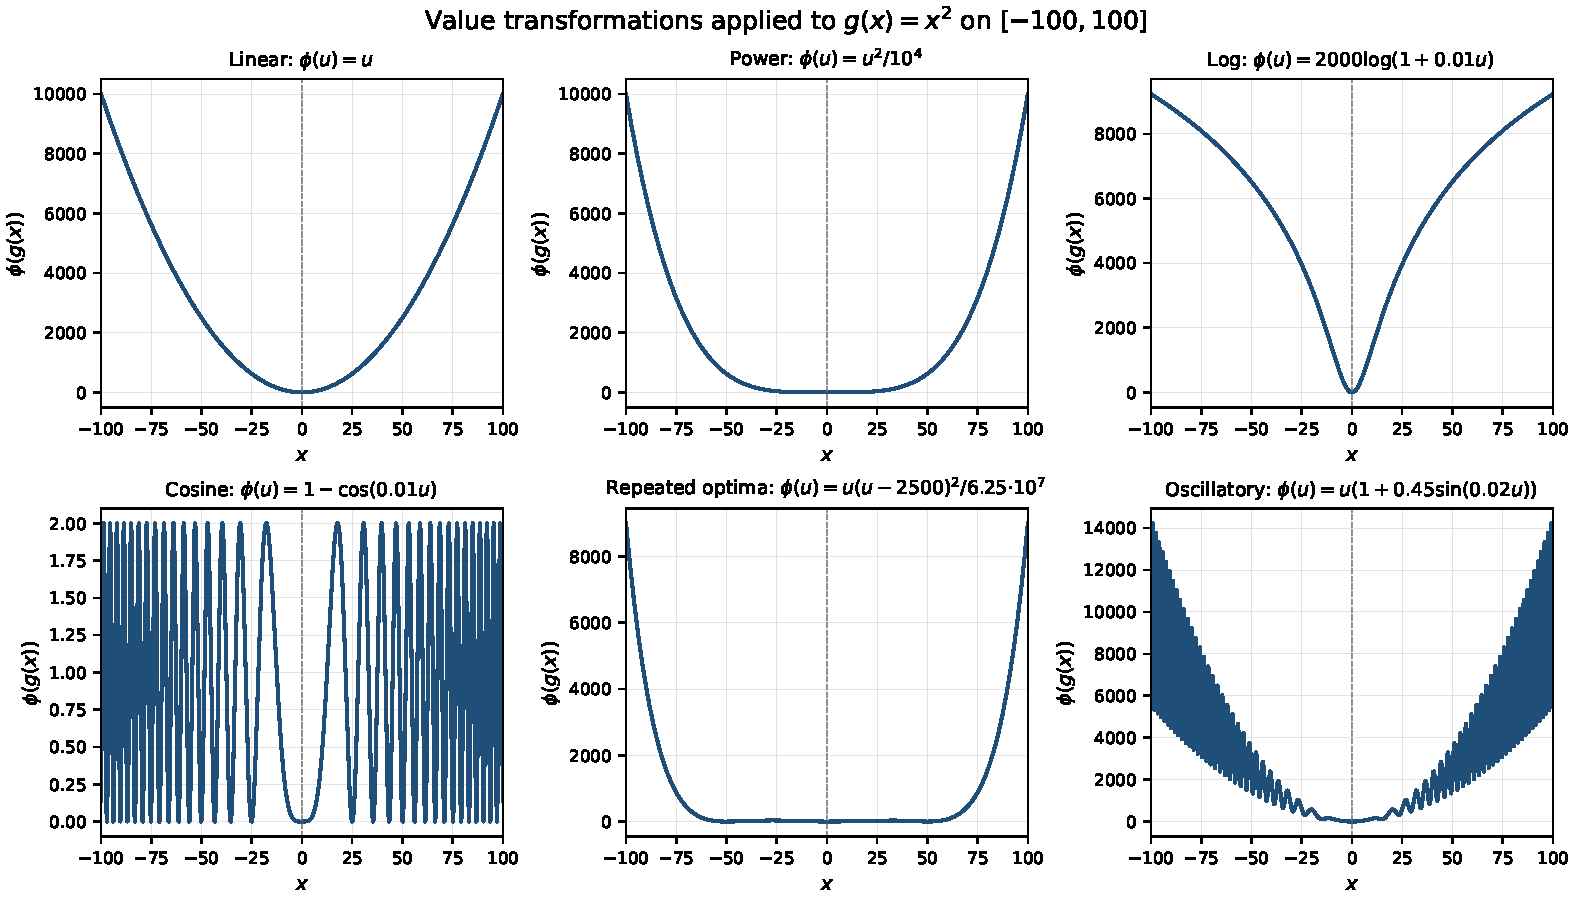
\includegraphics[width=\textwidth]{figures/value_transform_quadratic.pdf}
	\caption{Examples of value transformations applied to the same quadratic
	base function \(g(x)=x^2\) on \([-100,100]\). Each panel uses its own
	vertical scale to emphasize the induced shape.}
	\label{fig:value-transform-quadratic}
\end{figure}

In summary, strictly increasing value transformations preserve local minima and
only change shape. Nondecreasing transformations with flat intervals preserve
minimum values but can create plateaus and non-isolated minimizers. Nonmonotone
nonnegative transformations with \(\phi(0)=0\) preserve the known global optimum
while allowing additional local minima to appear at selected objective-value
levels. If \(\phi\) takes negative values on \(\mathbb{R}_{\ge0}\), then the
minimum-preservation argument no longer applies without a separate analysis.



\subsection{Composition function $\psi$}
\label{subsec:composition-function}

The composition function \(\psi\) combines the current point and the transformed
component values
\[
	z_i(x)=\phi_i(g_i(T_i(x))),
	\qquad
	z(x)=(z_1(x),\ldots,z_m(x)).
\]
Thus the final objective is
\[
	f(x)=\psi(x,z(x)).
\]
Equivalently, one may write \(\psi_x(z)=\psi(x,z)\). This notation is useful
when \(\psi\) uses spatial weights or gates. The \(x\)-independent case
\(\psi(x,z)=\psi(z)\) remains an important special case.

By design, \(\psi\) should preserve the known global minimum. For a prescribed
component-value vector \(v^\star=z(x^\star)\), the basic sufficient condition is
\[
	\psi(x^\star,v^\star)=0,
	\qquad
	\psi(x,z(x))\ge0
	\quad\text{for all }x\in\Omega.
\]

The local behavior follows from the chain rule. If \(z\) and \(\psi\) are
differentiable, then
\begin{equation}
	\nabla f(x)
	=
	\nabla_x\psi(x,z(x))
	+
	J_z(x)^T\nabla_z\psi(x,z(x)).
	\label{eq:composition-gradient}
\end{equation}
If both are twice differentiable, then
\begin{align}
	\nabla^2 f(x)
	={}&
	\nabla_{xx}^2\psi(x,z(x))
	+
	\nabla_{xz}^2\psi(x,z(x))J_z(x)
	+
	J_z(x)^T\nabla_{zx}^2\psi(x,z(x))
	\nonumber\\
	&+
	J_z(x)^T\nabla_{zz}^2\psi(x,z(x))J_z(x)
	+
	\sum_{i=1}^m
	\frac{\partial\psi}{\partial z_i}(x,z(x))\nabla^2 z_i(x).
	\label{eq:composition-hessian}
\end{align}
For an \(x\)-independent composition, the explicit-\(x\) terms vanish and
these formulas reduce to the usual chain-rule expressions involving only
derivatives with respect to \(z\).

The prescribed global minimizer is guaranteed by the value construction, not by
the differential formulas. The role of
\eqref{eq:composition-gradient} and \eqref{eq:composition-hessian} is instead
to describe how the composition changes the rest of the landscape. In
particular, local minimizers of the components are not automatically preserved.
At such a point, the component-value vector, the Jacobian \(J_z(x)\), and the
derivatives of \(\psi\) may all be different from their values at the prescribed
global minimizer. The full Hessian in
\eqref{eq:composition-hessian} contains the
\(J_z(x)^T\nabla_{zz}^2\psi(x,z(x))J_z(x)\) coupling term, the weighted
component Hessians, and any explicit-\(x\) terms. Therefore, a component-wise
local minimum can be weakened, removed, or reshaped by the composition unless
additional conditions on \(\psi\) and on the neighboring component landscapes
are imposed.

New stationary points can also be generated at the composition level. From
\eqref{eq:composition-gradient}, a point \(x_0\) is stationary whenever
\[
	\nabla_x\psi(x_0,z(x_0))
	+
	J_z(x_0)^T\nabla_z\psi(x_0,z(x_0))=0.
\]
This can happen even if the individual components are not all stationary. For
example, the component gradients may cancel after being weighted by
\(\nabla_z\psi(x_0,z(x_0))\), the explicit spatial derivative
\(\nabla_x\psi(x_0,z(x_0))\) may balance the component gradients, or \(\psi\)
may have a critical point at the reachable pair \((x_0,z(x_0))\). Such a
stationary point becomes a local minimum only when the composed value cannot
decrease in a neighborhood of \(x_0\). Therefore, composition can create local
minima through interaction among components, even when no single component
alone has a local minimum at that point.

\subsubsection{Same-point minimizers}

The simplest specialization is the case where all transformed components share
the same prescribed minimizer. Then the component-value vector at that point is
the zero vector, and the construction reduces to the common-minimizer case of
Proposition~\ref{thm:prescribed-point-construction}. The only additional
choice is to make \(\psi\) vanish at the zero component-value vector.

\begin{proposition}[Common-minimizer specialization]
	\label{cor:common-vanishing-construction}
	Assume that the value transformations follow
	Proposition~\ref{prop:minimum-preserving-value-transformations}, and choose
	a prescribed point \(x^\star\in\Omega\). If the coordinate transformations
	satisfy
	\[
	T_i(x^\star)=x_i^\star
	\qquad
	\text{for all }i=1,\ldots,m,
	\]
	and if \(\psi\) is chosen so that
	\[
	\psi(x^\star,0,\ldots,0)=0,
	\qquad
	\psi(x,z(x))\ge0
	\quad
	\forall x\in\Omega,
	\]
	then \(x^\star\) is a global minimizer of \(f\), and \(f(x^\star)=0\).
\end{proposition}

\begin{proof}
	This is the special case of
	Proposition~\ref{thm:prescribed-point-construction} with one prescribed
	point, \(r=1\), \(\tilde x_1=x^\star\), and assignment
	\(\sigma(i)=1\) for every component \(i=1,\ldots,m\). The condition
	\(T_i(x^\star)=x_i^\star\) is exactly
	\eqref{eq:prescribed-point-assignment} in this special case.
	
	Consequently, each component vanishes at \(x^\star\):
	\[
	g_i(T_i(x^\star))=g_i(x_i^\star)=0.
	\]
	Since \(\phi_i(0)=0\), the prescribed component vector is
	\[
	v^{(1)}=(0,\ldots,0).
	\]
	Therefore
	\[
	f(x^\star)=\psi(x^\star,0,\ldots,0)=0.
	\]
	The assumed nonnegativity of \(\psi(x,z(x))\) is the nonnegativity condition
	in Proposition~\ref{thm:prescribed-point-construction}. Hence the first
	statement of that proposition implies that \(x^\star\) is a global minimizer.
\end{proof}

When all components vanish at the same prescribed minimizer, the aggregation is
typically chosen to be nonnegative and nondecreasing in each component value. A
basic example is an \(x\)-dependent weighted sum,
\[
	\psi(x,z)=\sum_{i=1}^m w_i(x)z_i,
	\qquad
	w_i(x)\ge0.
\]
Note here that the weights only
need to be nonnegative. Normalization, such as \(\sum_i w_i(x)=1\), is not
required for minimum preservation; it only fixes the vertical scale. Constant
weights are recovered as the special case \(w_i(x)\equiv w_i\). Spatially
varying weights change which component dominates in different regions, and the
gradient contains additional terms \(z_i(x)\nabla w_i(x)\). These terms can
generate new stationary points by balancing component-value gradients against
weight gradients.

Other common aggregation choices include products,
\[
	\psi(x, z)=\prod_{i=1}^m(1+z_i)-1,
\]
and power means,
\[
	\psi(x,z)=
	\left(
	\sum_{i=1}^m \alpha_i(x) z_i^p
	\right)^{1/p},
	\qquad
	\alpha_i(x)\ge0,
	\quad
	p>0.
\]
Near the prescribed minimizer, the product behaves like a weighted sum with unit
weights, while away from the optimum it introduces multiplicative interactions
between components. Power means give a smooth value-dependent aggregation:
larger components receive more influence when \(p>1\). In both cases, new
stationary points can arise through weighted cancellation of component
gradients and through the additional Hessian terms introduced by the nonlinear
aggregation.

To deliberately generate new local minima from same-point unimodal components,
the value-dependent part of \(\psi\) may be chosen nonmonotone while remaining
nonnegative. A simple smooth example is
\[
	\psi(x,z)=s\left(1+\epsilon\sin(\alpha s)\right),
	\qquad
	s=\sum_{i=1}^m z_i,
	\qquad
	0<\epsilon<1.
\]
For a fixed positive \(\alpha\), this function satisfies \(\psi(0)=0\) and
\(\psi(z)>0\) for \(z\ne0\) in the nonnegative orthant, so the prescribed
global optimum is preserved. Allowing \(\alpha\) to depend on \(x\) gives a
spatially varying version of the same mechanism. In either case, \(\psi\) has
repeated stationary levels as a function of \(s\). Therefore, even if each
component \(z_i\) is convex and unimodal with the same minimizer, the
composition can become multimodal by creating local wells at positive
component-value levels.

Figure~\ref{fig:composition-functions-3d} illustrates these composition
functions on the domain \([-100,100]^2\), using two normalized two-dimensional
components: a Sphere and an Ellipsoid function, both convex, unimodal, and with
the same minimizer at the origin. The surfaces show how the same component
functions can produce different composed landscapes depending only on the
choice of the \(x\)-independent composition rule. In particular, the
nonmonotone level-well construction demonstrates that two convex unimodal
components with the same minimizer can still produce a multimodal composed
function. The height and color are based on \(\log(1+f)\), which makes both the
prescribed optimum and the large-scale landscape shape visible in the same
plot.

\begin{figure}[ht]
	\centering
	\includegraphics[width=\textwidth]{figures/composition_operators_3d.pdf}
	\caption{Three-dimensional examples of composition functions applied on
		\([-100,100]^2\) to two normalized two-dimensional components: a Sphere
		component and an Ellipsoid component. The surfaces use
		\(\log(1+f)\) as both height and color. The nonmonotone level-well example
		uses \(\psi(z)=s(1+0.65\sin(20s))\), where \(s=z_1+z_2\).}
	\label{fig:composition-functions-3d}
\end{figure}


\subsubsection{Deceptive point minimizers}

The local-minimum case in
Proposition~\ref{thm:prescribed-point-construction} gives the abstract
condition needed for a prescribed point to become locally attractive. This
subsubsection gives this case concrete mechanisms for enforcing the local condition.

A deceptive point is a suboptimal point that is locally attractive. In this
paper, we call \(\tilde x\) a deceptive point of \(f\) when \(\tilde x\) is a
local minimizer of \(f\), but
\[
	f(\tilde x)>f(x^\star),
\]
where \(x^\star\) is a known global minimizer. The construction below treats
deception as an add-on mechanism: first construct a function with a known global
optimum using the previous prescriptions, and then inject one or more local
basins with prescribed objective values. In this sense, the constructions in
this subsubsection are concrete ways to realize the local condition
\eqref{eq:prescribed-point-local-condition}.

\begin{proposition}[Construction of a deceptive point]
	\label{prop:add-on-deceptive-point}
	Let \(h:\Omega\to\mathbb{R}\) satisfy
	\[
	h(x^\star)=0,
	\qquad
	h(x)\ge0
	\qquad
	\forall x\in\Omega.
	\]
	Let \(g:\Omega_g\to\mathbb{R}\) be a base function with minimizer
	\(x_g^\star\), let \(\phi\) satisfy
	Proposition~\ref{prop:minimum-preserving-value-transformations}, and choose
	\(T:\Omega\to\Omega_g\) such that
	\[
	T(\tilde x)=x_g^\star.
	\]
	Let \(b>0\). Choose \(w_0,w_1:\Omega\to\mathbb{R}_{\ge0}\) such that
	\[
	w_0(x^\star)=1,
	\qquad
	w_1(x^\star)=0,
	\]
	and, for some neighborhood \(U\subset\Omega\) of \(\tilde x\),
	\[
	w_0(x)=0,
	\qquad
	w_1(x)=1
	\qquad
	\forall x\in U.
	\]
	Define
	\[
	q(x)=\phi(g(T(x)))+b,
	\qquad
	f(x)=w_0(x)h(x)+w_1(x)q(x).
	\]
	Then \(x^\star\) is a global minimizer of \(f\) with value \(0\), and
	\(\tilde x\) is a local minimizer of \(f\) with value \(b\). Hence
	\(\tilde x\) is a deceptive point.
\end{proposition}

\begin{proof}
	At the known global minimizer \(x^\star\),
	\[
	f(x^\star)
	=
	w_0(x^\star)h(x^\star)+w_1(x^\star)q(x^\star)
	=
	0.
	\]
	For every \(x\in\Omega\), the functions \(h\), \(q\), \(w_0\), and \(w_1\)
	are nonnegative. Therefore \(f(x)\ge0\), and
	Proposition~\ref{f_helper} implies that \(x^\star\) is a global minimizer of
	\(f\).
	
	On the neighborhood \(U\), the switching conditions give
	\[
	f(x)=q(x)=\phi(g(T(x)))+b.
	\]
	At the prescribed point,
	\[
	q(\tilde x)
	=
	\phi(g(T(\tilde x)))+b
	=
	\phi(g(x_g^\star))+b
	=
	b.
	\]
	For every \(x\in U\), \(g(T(x))\ge0\), and therefore
	\[
	q(x)=\phi(g(T(x)))+b\ge b=q(\tilde x).
	\]
	Thus \(f(\tilde x)\le f(x)\) for all \(x\in U\), so \(\tilde x\) is a local
	minimizer of \(f\). Since \(b>0=f(x^\star)\), the local minimizer is
	suboptimal.
\end{proof}

The single-point add-on in
Proposition~\ref{prop:add-on-deceptive-point} can also be written directly as a
composition function for the prescribed-point construction. The purpose is to
choose an \(x\)-dependent \(\psi\) that still satisfies
Proposition~\ref{thm:prescribed-point-construction}: it remains nonnegative,
maps one prescribed component vector to zero, and enforces the local condition
\eqref{eq:prescribed-point-local-condition} at the other prescribed points.
The weights provide this local enforcement by selecting the corresponding
component near each prescribed point, while the offsets determine which local
basin is global and which basins are deceptive.

\begin{proposition}[Deceptive weighted composition]
	\label{prop:deceptive-weighted-composition}
	For \(i=1,\ldots,m\), let \(g_i:\Omega_i\to\mathbb{R}\) be base functions
	with minimizers \(x_i^\star\), and let \(\phi_i\) satisfy
	Proposition~\ref{prop:minimum-preserving-value-transformations}.
	Choose prescribed points \(\tilde x_i\in\Omega\) and coordinate
	transformations \(T_i:\Omega\to\Omega_i\) such that
	\[
	T_i(\tilde x_i)=x_i^\star,
	\qquad
	i=1,\ldots,m.
	\]
	Let \(b_i\ge0\), and define
	\[
	z_i(x)=\phi_i(g_i(T_i(x))).
	\]
	Choose nonnegative weights \(w_i:\Omega\to\mathbb{R}_{\ge0}\), and define the
	\(x\)-dependent composition function
	\[
	\psi(x,z)
	=
	\sum_{i=1}^m w_i(x)(z_i+b_i),
	\qquad
	z=(z_1,\ldots,z_m).
	\]
	The generated function is
	\[
	f(x)=\psi(x,z(x))
	=
	\sum_{i=1}^m w_i(x)(z_i(x)+b_i).
	\]
	Assume that for each \(i\) there exists a neighborhood \(U_i\subset\Omega\)
	of \(\tilde x_i\) such that
	\[
	w_i(x)=1,
	\qquad
	w_j(x)=0\quad (j\ne i),
	\qquad
	\forall x\in U_i.
	\]
	Then each \(\tilde x_i\) is a local minimizer of \(f\), with
	\[
	f(\tilde x_i)=b_i.
	\]
	If one index \(k\) satisfies \(b_k=0\) and \(b_i>0\) for all \(i\ne k\), then
	\(\tilde x_k\) is a global minimizer of \(f\), and every \(\tilde x_i\) with
	\(i\ne k\) is a deceptive point. 
\end{proposition}

\begin{proof}
	Because \(w_i(x)\ge0\), \(z_i(x)=\phi_i(g_i(T_i(x)))\ge0\), and \(b_i\ge0\),
	the constructed composition satisfies
	\[
	\psi(x,z(x))\ge0
	\qquad
	\forall x\in\Omega.
	\]
	Thus the nonnegativity requirement in
	Proposition~\ref{thm:prescribed-point-construction} is satisfied.
	
	Fix \(i\). On the neighborhood \(U_i\), the switching conditions give
	\[
	f(x)=z_i(x)+b_i.
	\]
	At the prescribed point \(\tilde x_i\),
	\[
	z_i(\tilde x_i)+b_i
	=
	\phi_i(g_i(T_i(\tilde x_i)))+b_i
	=
	\phi_i(g_i(x_i^\star))+b_i
	=
	b_i.
	\]
	For every \(x\in U_i\), \(g_i(T_i(x))\ge0\), and therefore
	\[
	z_i(x)+b_i\ge b_i=f(\tilde x_i).
	\]
	Hence the local condition
	\eqref{eq:prescribed-point-local-condition} holds for \(\tilde x_i\), and
	Proposition~\ref{thm:prescribed-point-construction} implies that
	\(\tilde x_i\) is a local minimizer of \(f\), with value \(b_i\).
	
	If \(b_k=0\), then \(f(\tilde x_k)=0\). Since \(f(x)\ge0\) everywhere,
	the global-minimizer statement in
	Proposition~\ref{thm:prescribed-point-construction} applies with
	\(\tilde x_k\). If \(b_i>0\) for \(i\ne k\), then
	\(f(\tilde x_i)>f(\tilde x_k)\), so each \(\tilde x_i\) with \(i\ne k\) is
	suboptimal. Since these points are also local minimizers, they are deceptive
	points. 
\end{proof}

The weight functions determine how sharply the construction switches between
component basins. For the guarantee in
Proposition~\ref{prop:deceptive-weighted-composition}, the essential
requirements are nonnegativity and local selection: near each prescribed point
\(\tilde x_i\), the corresponding weight must be one and the other weights
must be zero. Normalization,
\[
	\sum_{i=1}^m w_i(x)=1,
\]
is useful for controlling scale, but it is not required for the minimum
arguments above. If the weights are normalized, then \(\psi(x,z)\) defines a local
or spatially varying blend of the shifted component objectives. 

Several choices for $w_i(x)$ are possible. Compactly supported bump functions can enforce
exact local selection, because one can set \(w_i=1\) on a small neighborhood of
\(\tilde x_i\) and smoothly taper it to zero outside a larger neighborhood.
Smooth approximate alternatives include distance-based softmax weights,
\[
	w_i(x)=
	\frac{\exp(-\alpha\|x-\tilde x_i\|^2)}
	{\sum_{j=1}^m \exp(-\alpha\|x-\tilde x_j\|^2)},
\]
inverse-distance weights of the form
\[
	w_i(x)=
	\frac{(\|x-\tilde x_i\|^2+\epsilon)^{-p}}
	{\sum_{j=1}^m(\|x-\tilde x_j\|^2+\epsilon)^{-p}},
\]
logistic gates for two-component transitions, and normalized
partition-of-unity weights \(w_i(x)=\eta_i(x)/\sum_j\eta_j(x)\) built from
nonnegative smooth basis functions \(\eta_i\). These smooth weights are easy to
implement, but they generally do not give exact zeros or ones. They therefore
approximate the ideal construction unless they are combined with local
hard-selection regions. Parameters such as \(\alpha\), \(p\), or the support
width of \(\eta_i\) control the sharpness of the transition: sharper weights
produce more localized basins but can also create steep transition regions.
These transition regions are not neutral, because the derivative of \(f\)
contains terms involving \((z_i(x)+b_i)\nabla w_i(x)\); consequently, the
choice of weights can itself create additional stationary points between
prescribed basins.

Figure~\ref{fig:deceptive-weighted-composition-3d} illustrates the construction
on \([-100,100]^2\) using three different pairs of base functions:
Rastrigin/Ellipsoid, Ackley/Rosenbrock, and Griewank/Sphere. In each panel, the
first component defines the global basin with offset \(b=0\), while the second
component defines a suboptimal deceptive basin with positive offset. The
weights select one component near each prescribed point and blend the
components away from these neighborhoods.

\begin{figure}[t]
	\centering
	\includegraphics[width=\textwidth]{figures/deceptive_weighted_composition_3d.pdf}
	\caption{Three-dimensional examples of deceptive weighted compositions on
		\([-100,100]^2\), using Rastrigin/Ellipsoid, Ackley/Rosenbrock, and
		Griewank/Sphere component pairs. In each panel, the white star marks the
		global minimizer induced by the first component, and the red point marks the
		suboptimal deceptive minimizer induced by the second component. Each surface
		uses \(\log(1+f)\) as both height and color.}
	\label{fig:deceptive-weighted-composition-3d}
\end{figure}


The local differential behavior follows the same logic as in the preceding
transformation and composition discussions. Inside a neighborhood \(U_i\) where
the switching conditions make \(w_i=1\) and \(w_j=0\) for \(j\ne i\), the
composed function reduces to
\[
	f(x)=z_i(x)+b_i=\phi_i(g_i(T_i(x)))+b_i.
\]
Thus, if \(\tilde x_i\) is an interior smooth basin minimum of the \(i\)-th
component, the Hessian at \(\tilde x_i\) is the Hessian of that transformed
component, scaled by \(\phi_i'(0)\), exactly as in the value- and
coordinate-transformation analyses. Away from these locally selected regions,
the derivatives of the weights also contribute. In particular, terms involving
\((z_i(x)+b_i)\nabla w_i(x)\) can create additional stationary points in
transition regions between basins. Hence the construction guarantees the
prescribed deceptive local minima, while the switching functions may introduce
further landscape structure.


\section{Code Implementation}
\subsection{Classification of Functions}

The framework can generate a very large number of benchmark functions because a
function is determined not only by the selected base functions, but also by the
coordinate transformations \(T_i\), value transformations \(\phi_i\),
composition function \(\psi\), dimensionality, number of components, and
numerical parameters. Therefore, generated functions should not be labeled by
assigning a new descriptive name to each instance. Instead, we use a structured
label that records the construction class, together with a separate metadata
record that stores the exact parameters.

The purpose of the classification is practical. It should allow users to group
functions by the construction choices that are expected to affect optimizer
behavior. For example, two functions may both be high-dimensional mixed
compositions with affine coordinate transformations and oscillatory value
transformations, even if they use different random rotations or different
parameter values. Such functions belong to the same construction class, but they
are different benchmark instances. The class label is therefore coarse enough
for benchmark-suite organization and result tables, while the instance metadata
is detailed enough for exact reproducibility.

The classification follows the same ingredients used to generate the function.
In \textsc{FuncCraft}, the base-function library contains \(N=28\) functions,
formed from the base functions used in CEC2014, CEC2017, and BBOB2009. A
generated benchmark instance is specified by a structural class and an instance
record,
\[
	\left(\mathcal{C},\mathcal{P},\mathcal{T},\mathcal{G};\theta\right).
\]
Here,
\[
\begin{array}{ll}
\mathcal{C} & \text{composition-function class},\\
\mathcal{P} & \text{value-transformation class},\\
\mathcal{T} & \text{coordinate-transformation class},\\
\mathcal{G} & \text{selected base functions}.
\end{array}
\]
The parameter record \(\theta\) stores the instance-specific choices, such as
dimension, number of components, random seed, rotations, shifts, weights,
prescribed points, and construction parameters. Thus the structural tuple is used
for grouping benchmark functions, while \(\theta\) is used for exact
reconstruction.

\begin{table}[t]
	\centering
	\small
	\caption{Initial classification dictionary for generated benchmark functions.}
	\label{tab:classification-dictionary}
	\begin{tabular}{p{0.13\textwidth}p{0.22\textwidth}p{0.55\textwidth}}
		\hline
		Class & Label & Meaning \\
		\hline
		\(\mathcal{C}\) & \texttt{NONE} &
		No composition; used only for a single component. \\
		\(\mathcal{C}\) & \texttt{CPM-SUM} &
		Common-point minimizer; constant nonnegative weights. \\
		\(\mathcal{C}\) & \texttt{CPM-PMEAN} &
		Common-point minimizer with power-mean aggregation. \\
		\(\mathcal{C}\) & \texttt{CPM-LWELL} &
		Common-point minimizer with level wells,
		\(\psi=s(1+\epsilon\sin(\alpha s))\). \\
		\(\mathcal{C}\) & \texttt{DPM-SOFTMAX} &
		Deceptive-point minimizer with distance-based softmax weights. \\
		\hline
		\(\mathcal{P}\) & \texttt{NONE} &
		No value transformation; \(\phi(u)=u\). \\
		\(\mathcal{P}\) & \texttt{COSZERO} &
		\(\phi(u)=1-\cos(\alpha u)\), which can create repeated zeros. \\
		\(\mathcal{P}\) & \texttt{OSC} &
		\(\phi(u)=u(1+\epsilon\sin(\alpha u))\), which preserves the zero
		while adding oscillatory structure. \\
		\(\mathcal{P}\) & \texttt{POWER} &
		\(\phi(u)=\alpha u^p\), with \(\alpha\) and \(p\) chosen to control
		flatness or sharpness near the optimum. \\
		\hline
		\(\mathcal{T}\) & \texttt{NONE} &
		No coordinate transformation; \(T_i(x)=x\) on the selected variables. \\
		\(\mathcal{T}\) & \texttt{ROT} &
		Rotation of the search coordinates. \\
		\(\mathcal{T}\) & \texttt{BLOCK} &
		Disjoint subspace selection; component subspaces have no overlap and
		their union covers all \(D\) variables. \\
		\(\mathcal{T}\) & \texttt{AFF} &
		General affine map \(T_i(x)=A_i(x-\bar{x})+x_i^\star\). \\
		\hline
	\end{tabular}
\end{table}

The labels in Table~\ref{tab:classification-dictionary} describe structural
choices only. Numerical values such as \(\alpha\), \(\epsilon\), \(p\), softmax
sharpness, rotations, affine matrices, subspace indices, and component weights
belong to \(\theta\). For example, two instances with the same
\((\mathcal{C},\mathcal{P},\mathcal{T},\mathcal{G})\) but different random
rotations or different level-well frequencies are in the same class, but they
are different benchmark instances.


\subsection{API}
\subsection{Figures}


\section{Conclusion}

This paper introduced a general framework for constructing scalable benchmark
functions from known base functions. The construction separates the benchmark
design into coordinate transformations, value transformations, and composition
functions. This separation makes the role of each ingredient explicit:
coordinate transformations control the geometry of the search space, value
transformations reshape individual component landscapes, and composition
functions determine how transformed components interact in the final objective.

The main theoretical contribution is a set of sufficient conditions that
preserve analytically known global optima. Starting from nonnegative base
functions with known minimum value zero, the framework gives prescriptions for
minimum-preserving value transformations, coordinate pullbacks, prescribed
points, same-point minimizers, nested constructions, and deceptive local
minimizers. These results provide a flexible way to generate benchmark
functions whose optima remain known while still allowing substantial control
over multimodality, conditioning, separability, repeated optima, local basin
structure, and deception.

The framework also gives a natural classification scheme for generated
functions. Instead of assigning a new name to every benchmark instance, a
generated function can be labeled by its composition-function class,
value-transformation class, coordinate-transformation class, selected base
functions, and parameter record. This makes large benchmark collections easier
to organize, reproduce, and analyze.

The proposed \textsc{FuncCraft} implementation is intended to make this
construction practical in C++ and Python. Large-scale empirical evaluation of
optimization algorithms on generated benchmark collections is left for future
work. Such studies can use the classification scheme developed here to assess
algorithm robustness across controlled families of landscape mechanisms rather
than only across a small fixed set of manually designed functions.















\bibliography{}

\appendix






\end{document}
